% Created 2021-09-11 Sat 09:35
% Intended LaTeX compiler: xelatex
\documentclass[letterpaper]{article}
\usepackage{graphicx}
\usepackage{grffile}
\usepackage{longtable}
\usepackage{wrapfig}
\usepackage{rotating}
\usepackage[normalem]{ulem}
\usepackage{amsmath}
\usepackage{textcomp}
\usepackage{amssymb}
\usepackage{capt-of}
\usepackage{hyperref}
\usepackage[margin=1in]{geometry}
\usepackage{fontspec}
\usepackage{indentfirst}
\setmainfont[ItalicFont = LiberationSans-Italic, BoldFont = LiberationSans-Bold, BoldItalicFont = LiberationSans-BoldItalic]{LiberationSans}
\newfontfamily\NHLight[ItalicFont = LiberationSansNarrow-Italic, BoldFont       = LiberationSansNarrow-Bold, BoldItalicFont = LiberationSansNarrow-BoldItalic]{LiberationSansNarrow}
\newcommand\textrmlf[1]{{\NHLight#1}}
\newcommand\textitlf[1]{{\NHLight\itshape#1}}
\let\textbflf\textrm
\newcommand\textulf[1]{{\NHLight\bfseries#1}}
\newcommand\textuitlf[1]{{\NHLight\bfseries\itshape#1}}
\usepackage{fancyhdr}
\pagestyle{fancy}
\usepackage{titlesec}
\usepackage{titling}
\makeatletter
\lhead{\textbf{\@title}}
\makeatother
\rhead{\textrmlf{Compiled} \today}
\lfoot{\theauthor\ \textbullet \ \textbf{2021-2022}}
\cfoot{}
\rfoot{\textrmlf{Page} \thepage}
\titleformat{\section} {\Large} {\textrmlf{\thesection} {|}} {0.3em} {\textbf}
\titleformat{\subsection} {\large} {\textrmlf{\thesubsection} {|}} {0.2em} {\textbf}
\titleformat{\subsubsection} {\large} {\textrmlf{\thesubsubsection} {|}} {0.1em} {\textbf}
\setlength{\parskip}{0.45em}
\renewcommand\maketitle{}
\author{Houjun Liu}
\date{\today}
\title{Central Dogma, Protein Synthesis}
\hypersetup{
 pdfauthor={Houjun Liu},
 pdftitle={Central Dogma, Protein Synthesis},
 pdfkeywords={},
 pdfsubject={},
 pdfcreator={Emacs 27.2 (Org mode 9.4.4)}, 
 pdflang={English}}
\begin{document}

\maketitle


\section{Central Dogma}
\label{sec:orge00fb32}
Central dogma is the concept that the instructions of protein synthesis
comes from the DNA, and that DNA creates RNA creates Protein, RNA
creates RNA, DNA creates DNA, but this flow path could not be reversed.

We know a little bit more about central dogma now, and now have more
concise operations for the processes defined in the central dogma,
namely\ldots{}

\begin{itemize}
\item \textbf{DNA Polymerase} takes DNA and makes more DNA

\begin{itemize}
\item Duplicates cell DNA
\item Could be hijacked during cell cycle to duplicate DNA viruses
\item DNA viruses may also carry their DNA Polymerease to not wait for the
cell cycle
\end{itemize}

\item \textbf{RNA Polymerease} takes DNA and makes mRNA

\begin{itemize}
\item Have lower fidelity with an error about 1/100,000
\item Hence why safety mechanism needed
\end{itemize}
\end{itemize}

\subsection{Protein Synthesis}
\label{sec:orgf9f9378}
See \href{KBhBIO101ProteinSynthesis.org}{KBhBIO101ProteinSynthesis}

Eukarotic gene expression is regulated at many stages because mRNA is
pretty error-prone and so there needs to be many different steps

\begin{figure}[htbp]
\centering
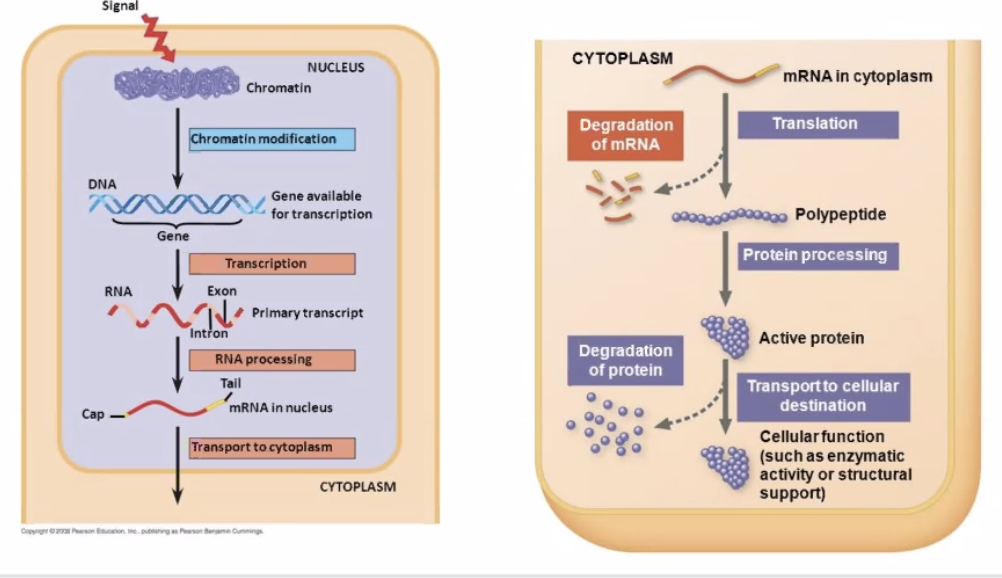
\includegraphics[width=.9\linewidth]{preprocessing.png}
\caption{preprocessing.png}
\end{figure}

\subsection{DNA Replication}
\label{sec:orgfe0e307}
See \href{KBhBIO101DNAReplication.org}{KBhBIO101DNAReplication}

\subsection{RNA Replication}
\label{sec:orgbda1179}
See \href{KBhBIO101RNAReplication.org}{KBhBIO101RNAReplication}

\subsection{List of Kool Proteins}
\label{sec:orgaab9ac1}
\begin{center}
\begin{tabular}{ll}
Name & Function\\
\hline
RNA Polymerase & \emph{transcripts}: takes DNA and turns into mRNA\\
DNA Polymerase & \emph{replicates}: takes DNA and makes more copy of it\\
RNA-Dependent RNA Polymerase & \emph{replicates}: takes RNA and makes more copy of it. Basically only viruses use it.\\
Promoter & \emph{signals}: DNA signal of the start of the DNA.\\
Terminator & \emph{signals}: DNA signal of the end of the DNA.\\
\end{tabular}
\end{center}

\noindent\rule{\textwidth}{0.5pt}

\section{Central Dogma in a Paragraph}
\label{sec:orgcbe9195}
The "silly" explanation of the Central Dogma that's a bit problematic is
the phrase "DNA" informs "RNA" informs "Proteins". But of course the
enviromental variablity, mutatability, and the surprising lack of
permanence of all parts of this system makes this not entirely fully
accurate.

DNA could of course replicate, that's how one makes new cells. But in
addition to this, during the process of transcription, there are also
enviromental variations to the performance of promoters, etc.
\end{document}
